\chapter{5.Entrauschen: Filter und Co}
%This, again, is just a translation of my lecture note
%TODO move the tikz graphics into the dedicated directory
    \subsection{Noise}
        \mim{Noise}: Unwanted disturbances in an image
        \begin{enumerate}[-]
            \item point wise
            \item random
            \item independent
            \item additive (for multiplicative noise use $log$)
        \end{enumerate}

        Notation:
        \begin{center}
            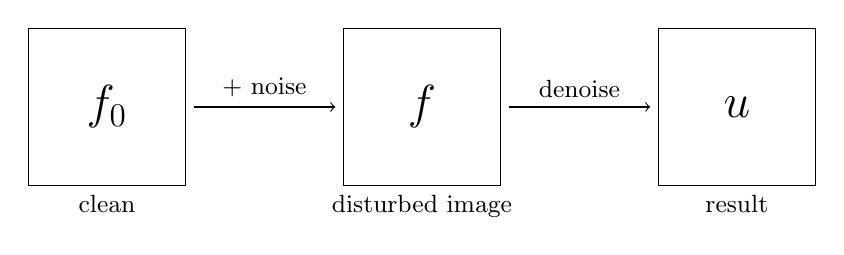
\begin{tikzpicture}
                \draw (0,0) rectangle (2,2);
                \draw (1,0) node[below] {\small clean};
                \draw (1,1) node[] {\LARGE $f_0$};
                \draw[->] (2.1,1) -- node[above] {\small $+$ noise} (3.9,1);
                \draw (4,0) rectangle (6,2);
                \draw (5,0) node[below] {\small disturbed image};
                \draw (5,1) node[] {\LARGE $f$};
                \draw[->] (6.1,1) -- node[above] {\small denoise} (7.9,1);
                \draw (8,0) rectangle (10,2);                
                \draw (9,0) node[below] {\small result};
                \draw (9,1) node[] {\LARGE $u$};
            \end{tikzpicture}
        \end{center}

        The quality of the denoised image $u$ compared to the original image $f_0$ is described by norms.
        \[\norm{f-f_0}, \text{noise}\]
        \[\norm{u-f_0}, \text{\mim{absolute error}}\]
        \[\frac{\norm{u-f_o}}{\norm{f-f_0}}, \text{\mim{relative error} compared to the noise}\]
        \[\frac{\norm{u-f_o}}{\norm{f_0}}, \text{relative error compared to the signal}\]
        
        Typically the chosen norm is:
        \[\norm{f} = \norm{f}_2 = \sqrt{\int_{\Omega} \abs{f(x)}^2 dx}\]
        or in the discrete:
        \[\norm{f}_2=\sqrt{\sum_{x \in \Omega} \abs{f(x)}^2}\]

        Closely connected is the \mim{Signal to noise ratio} (SNR):
        \[log(\underbrace{\frac{\norm{f_0}_2}{\norm{u-f_0}_2}}_{\in \ [1,\infty)}) \in [0,+\infty), \text{ where $0$ is bad and $+\infty$ is good.}\]
    \subsection{smoothing filter}
        Idea: (to simplify in 1D)
        \begin{center}
            \begin{tikzpicture}
                \draw (0,0) node[left] {$f_0$:};
                \draw[thick] plot [smooth, tension = 0.7] coordinates {(0,0) (1.75,1.5) (3.5,0.5) (6,2) (9,0) (11,0.5)};
                \draw[->,thick] (-0.3,-0.5) -- node[left] {noise} (-0.3,-2);
                \draw (0,-2.5) node[left] {$f$:};                
                \draw[thick, name path = P2,shift = {(0,-2.5)}] plot [smooth, tension = 0.7] coordinates {(0,0) (1.75,1.5) (3.5,0.5) (6,2) (9,0) (11,0.5)};
                \draw[name path = P1, draw = none] (0,-1.1) -- (3,-1.1);
                \draw[name intersections={of = P1 and P2},red,thick]
                (intersection-1) edge[bend right] ++(0.3,0.5) ++(0.3,0.5) edge[bend right] (intersection-2);
                \draw[name path = P3,draw = none] (3,-2.3) -- (5,-1.2);
                \draw[name intersections={of = P3 and P2},red,thick]
                (intersection-1) edge[bend left] ++(0.3,-0.3) ++(0.3,-0.3) edge[bend left] (intersection-2);
                \draw[] (2,-0.9) -- ++(0.5,-0.1) node[right] {\small disturbances} (3.5,-2.1) -- ++(-0.5,0.9);
                \draw (0,-5) node[left] {$f$:};
                \draw[thick, name path = P4,shift = {(0,-5)}] plot [smooth, tension = 0.7] coordinates {(0,0) (1.75,1.5) (3.5,0.5) (6,2) (9,0) (11,0.5)};
                \draw[name path = P5, shift = {(0,-2.5)}, draw = none] (0,-1.1) -- (3,-1.1);
                \draw[name intersections={of = P4 and P5},red,thick]
                (intersection-1) edge[bend right] node[black,pos=0] {\small \textbullet} ++(0.3,0.5) ++(0.3,0.5) edge[bend right] node[black,pos=1] {\small \textbullet}  node[black,pos=0] {\small \textbullet} (intersection-2);
                \draw[name path = P6, shift = {(0,-2.5)}, draw = none] (3,-2.3) -- (5,-1.2);
                \draw[name intersections={of = P4 and P6},red,thick]
                (intersection-1) edge[bend left] node[black,pos=0] {\small \textbullet} ++(0.3,-0.3) ++(0.3,-0.3) edge[bend left] node[black,pos=1] {\small \textbullet}  node[black,pos=0] {\small \textbullet} (intersection-2);
                \draw[decorate,decoration={brace,amplitude=2pt,mirror}] (1.4,-3.7) -- (2.2,-3.7);
                \draw[thick] (1.8,-3.8) -- (1.8,-4.3) node[below] {\small \framebox{average}};
                \draw[->,thick,double] (1.6,-5) -- (0.4,-5);
                \draw[->,thick,double] (2,-5) -- (3.2,-5);
                \draw[->,thick] (1.8,-5.1) -- (1.8,-5.7);
                \draw (0,-7.5) node[left] {$u$:};
                \draw[->,thick] (-0.3,-5.5) -- node[left] {denoising} (-0.3,-7);
                \draw[thick, name path = P7,shift = {(0,-7.5)}] plot [smooth, tension = 0.7] coordinates {(0,0) (1.75,1.5) (3.5,0.5) (6,2) (9,0) (11,0.5)};
                \draw[name path = P8, shift = {(0,-5)}, draw = none] (0,-1.2) -- (3,-1.2);
                \draw[name intersections={of = P7 and P8},red,thick]
                plot [smooth,tension=0.7] coordinates {(intersection-1) ($(intersection-1) + (0.5,0.35)$) (intersection-2)};
                \draw[name path = P9, shift = {(0,-5)}, draw = none] (3,-2.25) -- (5,-1.15);
                \draw[name intersections={of = P7 and P9},red,thick]
                plot [smooth,tension=0.7] coordinates {(intersection-1) ($(intersection-1) + (0.45,0.05)$) (intersection-2)};
            \end{tikzpicture}
        \end{center}

        \begin{equation} \label{eq:5.1}
            u(k):=\alpha \cdot f(k-1) + \beta \cdot f(k) + \gamma \cdot f(k+1)
        \end{equation}
        where:
        \begin{equation} \label{eq:5.2}
            \alpha + \beta + \gamma = 1
        \end{equation}

        More precisely \eqref{eq:5.1} means:
        
        \begin{center}
            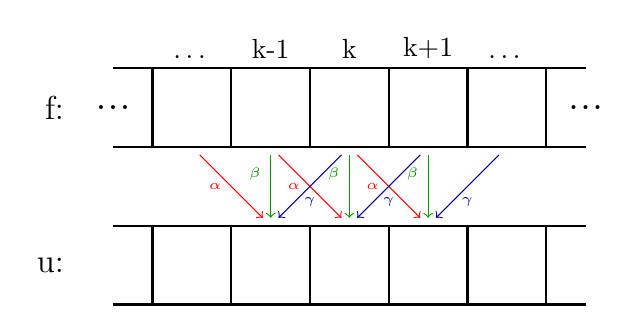
\begin{tikzpicture}
                \draw (0,-0.5) node[left] {\large f:};
                \draw[thick] (0.5,0) grid (6.5,-1);
                \draw (0.5,-0.5) node {\LARGE ...};
                \draw (6.5,-0.5) node {\LARGE ...};
                \draw (1.5,0) node[above] {\dots};
                \draw (2.5,0) node[above] {k-1};
                \draw (3.5,0) node[above] {k};
                \draw (4.5,0) node[above] {k+1};
                \draw (5.5,0) node[above] {\dots};

                \draw[->,red] (1.6,-1.1) -- node[left] {\tiny $\alpha$} (2.4,-1.9);
                \draw[->,red] (2.6,-1.1) -- node[left] {\tiny $\alpha$} (3.4,-1.9);
                \draw[->,red] (3.6,-1.1) -- node[left] {\tiny $\alpha$} (4.4,-1.9);
                \draw[->,black!40!green] (2.5,-1.1) -- node[left, pos = 0.3] {\tiny $\beta$} (2.5,-1.9);
                \draw[->,black!40!green] (3.5,-1.1) -- node[left, pos = 0.3] {\tiny $\beta$} (3.5,-1.9);
                \draw[->,black!40!green] (4.5,-1.1) -- node[left, pos = 0.3] {\tiny $\beta$} (4.5,-1.9);
                \draw[->,black!40!blue] (3.4,-1.1) -- node[right, pos = 0.75] {\tiny $\gamma$} (2.6,-1.9);
                \draw[->,black!40!blue] (4.4,-1.1) -- node[right, pos = 0.75] {\tiny $\gamma$} (3.6,-1.9);
                \draw[->,black!40!blue] (5.4,-1.1) -- node[right, pos = 0.75] {\tiny $\gamma$} (4.6,-1.9);

                \draw (0,-2.5) node[left] {\large u:};
                \draw[thick] (0.5,-2) grid (6.5,-3);
            \end{tikzpicture}
        \end{center}

        \begin{center}
            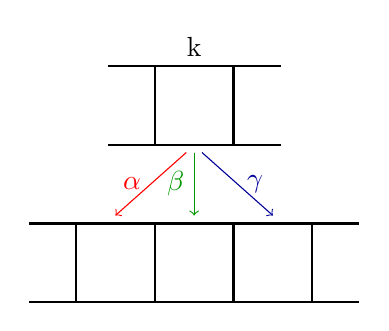
\begin{tikzpicture}
                \draw (0.5,0) node[above] {k};
                \draw[thick] (-0.6,0) grid (1.6,-1);
                \draw[->,red] (0.4,-1.1) -- node[left] {$\alpha$} (-0.5,-1.9);
                \draw[->,black!40!green] (0.5,-1.1) -- node[left] {$\beta$} (0.5,-1.9); 
                \draw[->,black!40!blue] (0.6,-1.1) -- node[right] {$\gamma$} (1.5,-1.9); 
                \draw[thick] (-1.6,-2) grid (2.6,-3);
            \end{tikzpicture}
        \end{center}

		With \eqref{eq:5.1} there is a mapping $f \mapsto u$, we write
		\[u = m \boxast f, \ \text{this is called \mim{Correlation}.}\]%TODO is it really correlation?
		where:
        \begin{equation}\label{eq:5.3}
            \framebox{$\displaystyle (m \boxast f)(k) = \sum_{i \in supp(m)} m(i) f(k+i)$}
        \end{equation}
        and:
        \begin{center}
            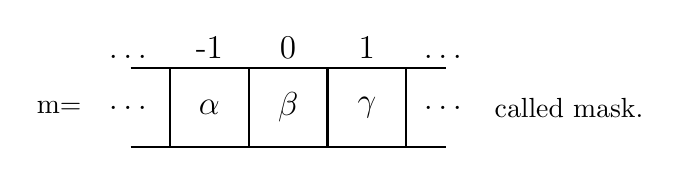
\begin{tikzpicture}
                \draw (0,0.5) node[left] {m=};
                \draw[thick] (0.5,0) grid (4.5,1);
                \draw (0.5,0.5) node {\large \dots};
                \draw (1.5,0.5) node {\large $\alpha$};
                \draw (2.5,0.5) node {\large $\beta$};
                \draw (3.5,0.5) node {\large $\gamma$};                
                \draw (4.5,0.5) node {\large \dots};
                \draw (0.5,1) node[above] {\large \dots};
                \draw (1.5,1) node[above] {\large -1};
                \draw (2.5,1) node[above] {\large 0};
                \draw (3.5,1) node[above] {\large 1};                
                \draw (4.5,1) node[above] {\large \dots};
                \draw (5,0.5) node[right] {called \mim{mask}.};
            \end{tikzpicture}
        \end{center}

        If you set $j:= k + i$ in \eqref{eq:5.1}, then $i=j-k$, which means:
        \begin{equation}\label{eq:5.4}
            \framebox{$\displaystyle (m \boxast f)(k) = \sum_{i \in supp(m)} m(j-k) f(j)$}
        \end{equation}

        To apply the mapping onto the boundary the image is reflected, in 1D:
        \begin{center}
            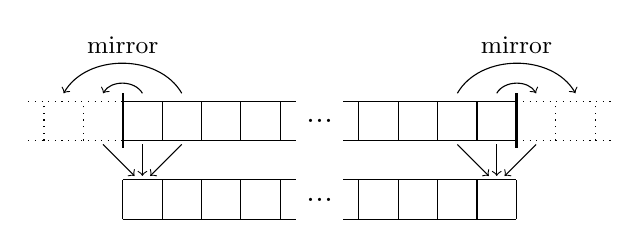
\begin{tikzpicture}
                \draw[step = 0.5] (0,0) grid (2.2,-0.5);
                \draw (2.5,-0.25) node {\large ...};
                \draw[step = 0.5] (2.8,0) grid (5,-0.5);
                \draw[thick] (0,0.1) -- (0,-0.6);
                \draw[thick] (5,0.1) -- (5,-0.6);
                \draw[step = 0.5, dotted] (0,0) grid (-1.2,-0.5);
                \draw[step = 0.5, dotted] (5,0) grid (6.2,-0.5);
                \draw[] (0.25,0.1) edge[bend right = 60, ->] (-0.25,0.1);
                \draw[] (0.75,0.1) edge[bend right = 60, ->] node[above] {\small mirror} (-0.75,0.1);
                \draw[] (4.75,0.1) edge[bend left = 60, ->] (5.25,0.1);
                \draw[] (4.25,0.1) edge[bend left = 60, ->] node[above] {\small mirror} (5.75,0.1);
                \draw[step = 0.5] (0,-1) grid (2.2,-1.5);
                \draw (2.5,-1.25) node {\large ...};
                \draw[step = 0.5] (2.8,-1) grid (5,-1.5);
                \draw[->] (0.25,-0.55) -- (0.25,-0.95);
                \draw[->] (-0.25,-0.55) -- (0.15,-0.95);
                \draw[->] (0.75,-0.55) -- (0.35,-0.95);
                \draw[->] (4.75,-0.55) -- (4.75,-0.95);
                \draw[->] (4.25,-0.55) -- (4.65,-0.95);
                \draw[->] (5.25,-0.55) -- (4.85,-0.95);
            \end{tikzpicture}
        \end{center}

        in 2D:

        \begin{center}
            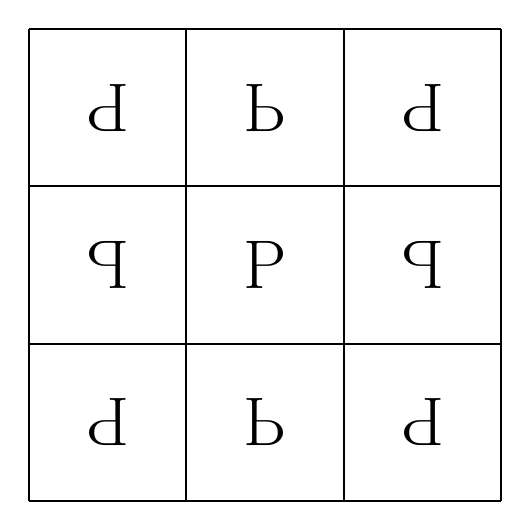
\begin{tikzpicture}
                \draw[step =2, thick] (0,0) grid (6,6);
                \draw (3,3) node {\Huge P};
                \draw (1,1) node[rotate = 180] {\Huge P};
                \draw (5,1) node[rotate = 180] {\Huge P};
                \draw (1,5) node[rotate = 180] {\Huge P};
                \draw (5,5) node[rotate = 180] {\Huge P};
                \draw (3,5) node[yscale=-1,xscale=1] {\Huge P};
                \draw (5,3) node[rotate = 180,yscale=-1,xscale=1] {\Huge P};
                \draw (1,3) node[rotate = 180,yscale=-1,xscale=1] {\Huge P};
                \draw (3,1) node[yscale=-1,xscale=1] {\Huge P};
            \end{tikzpicture}
        \end{center}

        Formula \eqref{eq:5.4} might remind one of the \mim{convolution}:
        \begin{equation}\label{eq:5.5}
            \framebox{$\displaystyle (g * f)(k) = \sum_{j \in \Z} g(\underbrace{k-j}_{\text{Difference to \eqref{eq:5.4}}}) \cdot f(j)$}
        \end{equation}

        If you set $g(i) := m(-i) =: \tilde m(i)$, which corresponds to a reflection of the Mask, then
        \[m \boxast f = g * f = \tilde m * f\]

        Properties of the convolution:
        \begin{enumerate}
            \item $(f * g) * h = f * (g* h)$, Associativity
            \item $f*g=g*f$, Commutativity
            \item $\tilde f * \tilde g = \widetilde{f * g}$, Compatibility with reflection
        \end{enumerate}
        
        Properties of the correlation:
        \begin{enumerate}
            \item $f \boxast (g \boxast h) = \tilde f * ( \tilde g* h) \overset{\framebox{\small 1}}{=} ( \tilde f * \tilde g) * h \overset{\framebox{\small 3}}{=} (\widetilde{f * g}) * h = (f * g) \boxast h \neq (f \boxast g) \boxast h$, not associative!
            \item $f \boxast g = \tilde f * g \overset{\framebox{\small 2}}{=} g * \tilde f = \tilde{\tilde g} * \tilde f \overset{\framebox{\small 3}}{=} \widetilde{(\tilde g * f)} = \widetilde{g \boxast f} \neq g \boxast f$, not commutative!
            \item $\tilde f \boxast \tilde g = \tilde{\tilde f} * \tilde g \overset{\framebox{\small 3}}{=} \widetilde{(\tilde f * g)} = \widetilde{f \boxast g}$, Compatibility with reflection
        \end{enumerate}